\subsection{Wave number}

Wave number is a measure of the number of waves per unit distance. It is inversely proportional to wave speed.Hourly observations are collected for the month of October 2015 using an Argus video monitoring system mounted on shore. Photogrammetry is performed on the video to determine the dominant wave frequencies and wave numbers in the survey area \citep{holman2013}. Data is available for a 2-dimensional area at the FRF survey site. A 1-dimensional profile is extracted from the 2-dimensional data along a transect corresponding to the position of the model boundary point. Figure~\ref{k1Dmean} shows statistics for wave number, \textit{k}, along the transect for October 2015. Wave number is shown to be more variable over time further from the coastline. Mean wave number decreases toward the shoreline, as expected.



\begin{figure}[h]
\centering
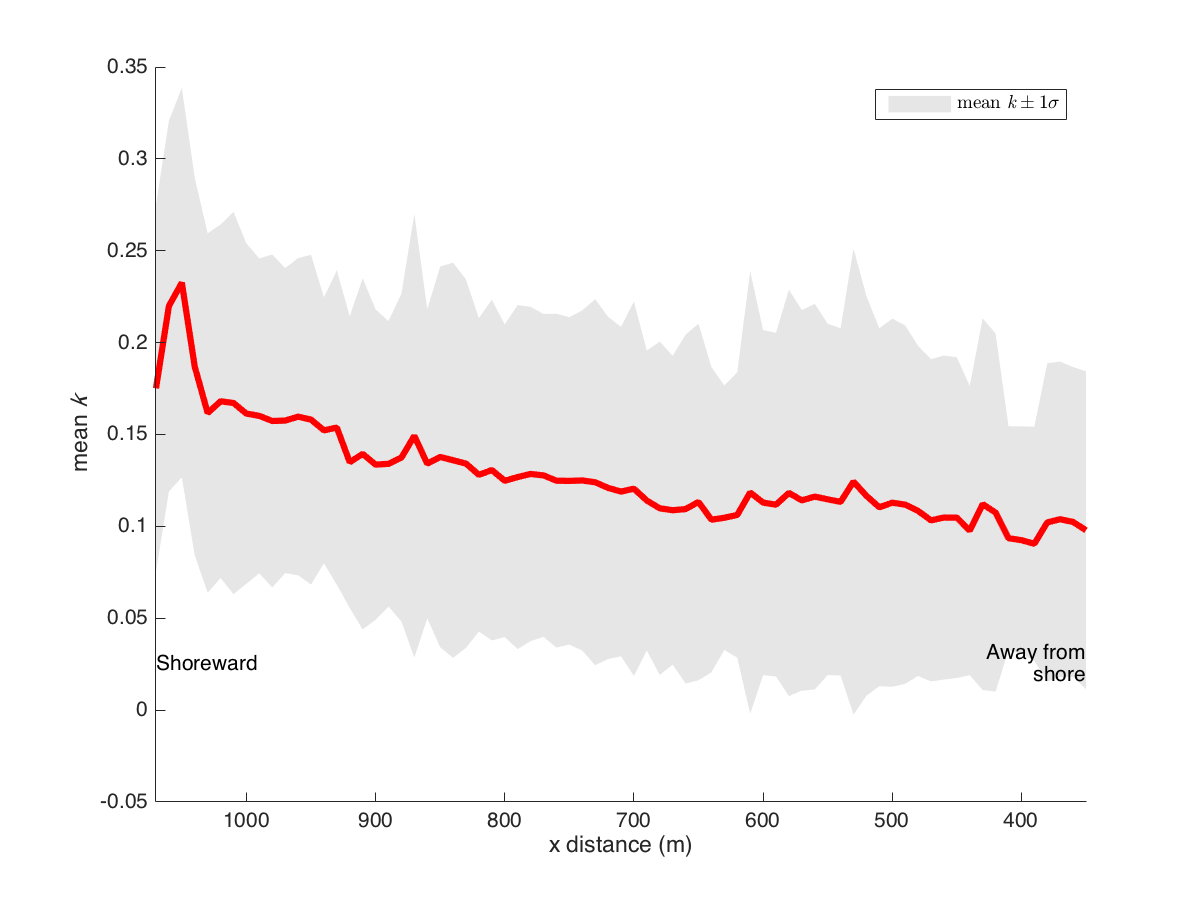
\includegraphics[width=.55\linewidth]{img/k1Dmean_std.png}
\caption{Wave number along the profile where the model boundary condition is located. Mean wave number, \textit{k}, during October 2015 is shown in red. Gray envelopes show $\pm$ 1$\sigma$ standard deviation in \textit{k}. Wave number is observed to be relatively larger and more variable further from shore.}
\label{k1Dmean}
\end{figure}